\section{BC05 - Industrialisation d'un algorithme d'apprentissage automatique et automatisation des processus de décision}

\begin{frame}
    \centering
    \huge
    BC05 - Industrialisation d'un algorithme d'apprentissage automatique et automatisation des processus de décision
\end{frame}

\begin{frame}{Architecture de déploiement}
	\begin{columns}[T]
		\column{0.69\textwidth}
		
		\vspace{-0.4cm}
		
		\begin{figure}[c]
			\centering
			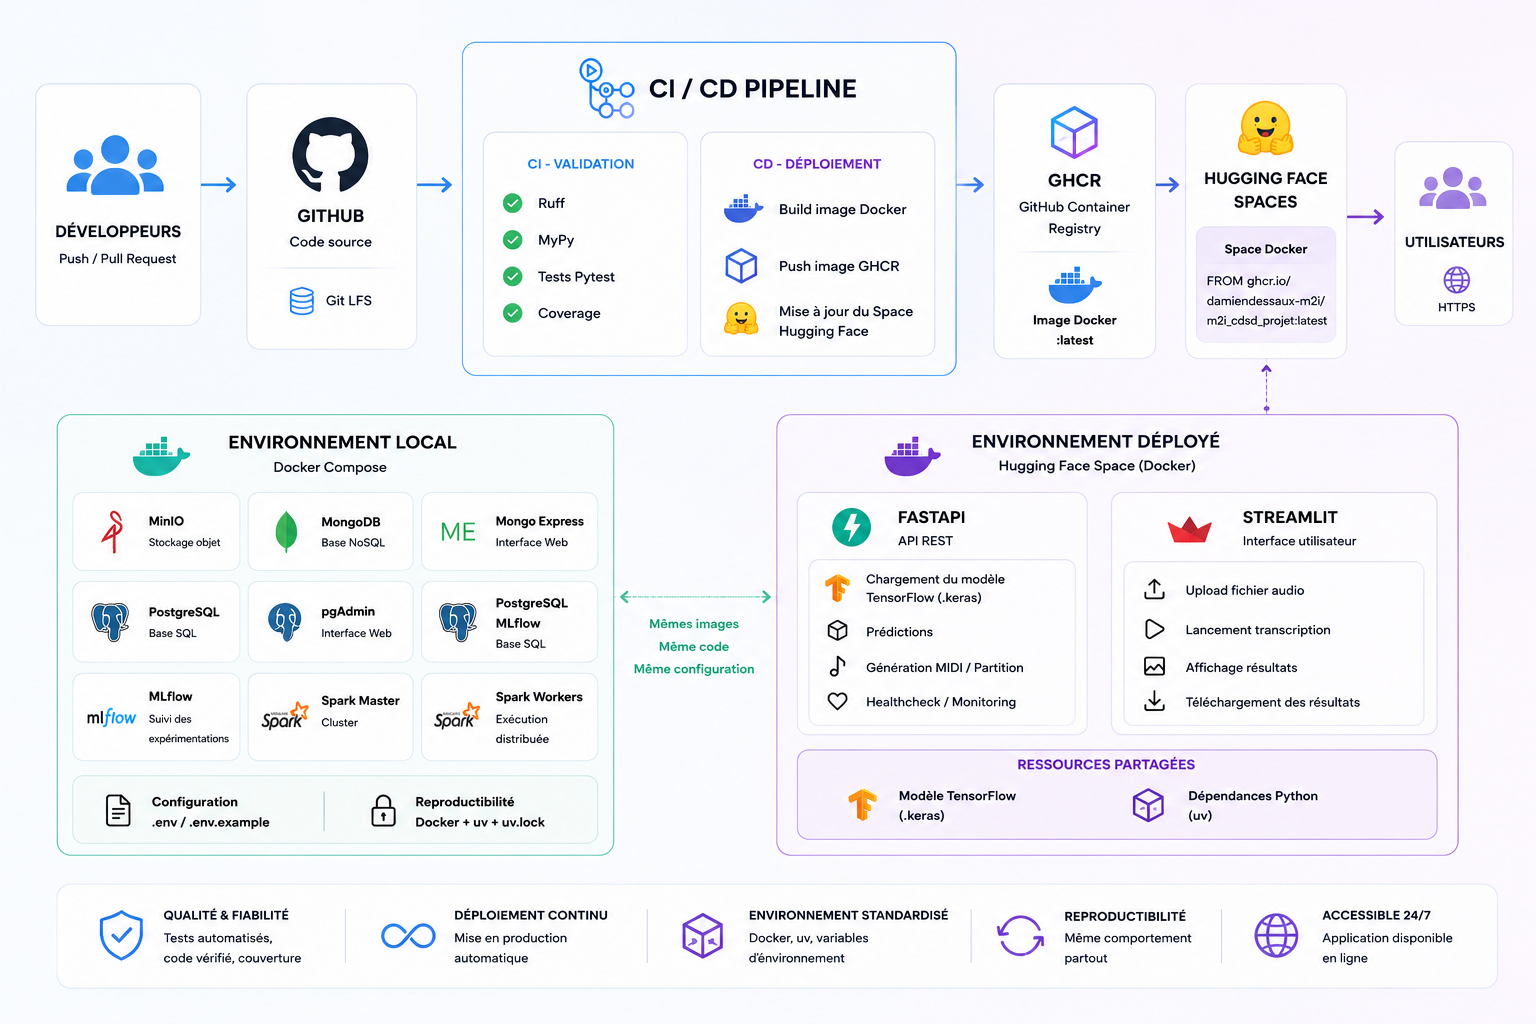
\includegraphics[height=0.8\textheight]{figures/BC05/cicd_deployment_architecture.png}
			% \caption{}
			\label{fig:cicd_deployment_architecture}
		\end{figure}
		
		\column{0.3\textwidth}
		
		\small
		\textbf{Pipeline de déploiement}
		\begin{itemize}
			\item Sélection du meilleur modèle et intégration à l'API.
			\item CI valide la qualité du projet.
			\item CD construis l'image Docker et la publie sur GHCR.
			\item Mise à jour du Space Hugging Face.
		\end{itemize}
		
		\begin{block}{\small Conclusion}
			\small Environnement d'exécution identique entre développement, CI/CD et production.
		\end{block}
	\end{columns}
\end{frame}

\begin{frame}[fragile]{Standardisation de l'environnement}
	\begin{columns}[T]
		\column{0.36\textwidth}
		
		\textbf{Environnement reproductible}
		\begin{itemize}
			\item Docker
			\item \texttt{pyproject.toml}
			\item \texttt{uv.lock}
			\item dépendances versionnées
		\end{itemize}
		
		\vspace{0.2cm}
		
		\textbf{Optimisation}
		\begin{itemize}
			\item Dockerfile multi-stage
			\item utilisateur non privilégié
		\end{itemize}
		
		\begin{block}{Résultat}
		L'utilisation conjointe de Docker et uv garantit un environnement standardisé, reproductible et portable.
		\end{block}
		
		\column{0.6\textwidth}
		
		\begin{lstlisting}[style=tinyterminal,language=python]
FROM ghcr.io/astral-sh/uv:python3.13-bookworm-slim AS builder
WORKDIR /app
ENV UV_COMPILE_BYTECODE=1 UV_LINK_MODE=copy UV_NO_CACHE=1
COPY pyproject.toml uv.lock ./
RUN uv sync --frozen --no-dev --group api
COPY api/backend ./backend
COPY api/frontend ./frontend
COPY api/.streamlit ./.streamlit
COPY api/start.sh ./start.sh

FROM python:3.13-slim-bookworm AS runtime
WORKDIR /app
RUN apt-get update && apt-get install -y --no-install-recommends libsndfile1 libcairo2 && rm -rf /var/lib/apt/lists/*
ENV PYTHONUNBUFFERED=1 PYTHONDONTWRITEBYTECODE=1 PATH="/app/.venv/bin:${PATH}"
COPY --from=builder /app/.venv ./.venv
COPY --from=builder /app/backend ./backend
COPY --from=builder /app/frontend ./frontend
COPY --from=builder /app/.streamlit ./.streamlit
COPY --from=builder /app/start.sh ./start.sh
RUN chmod +x start.sh
RUN mkdir -p /tmp
RUN useradd --create-home --shell /usr/sbin/nologin appuser && chown -R appuser:appuser /app && chmod 777 /tmp
USER appuser
EXPOSE 7860
EXPOSE 8000
HEALTHCHECK --interval=30s --timeout=5s --start-period=20s --retries=3 CMD python -c "import urllib.request; urllib.request.urlopen('http://127.0.0.1:8000/health')" || exit 1
CMD ["./start.sh"]
\end{lstlisting}
	\end{columns}
\end{frame}

%\begin{frame}{Standardisation de l'environnement}
%	\begin{columns}[T]
%		\column{0.48\textwidth}
%		
%		\textbf{Environnement reproductible}
%		\begin{itemize}
%			\item Docker
%			\item \texttt{pyproject.toml}
%			\item \texttt{uv.lock}
%			\item dépendances versionnées
%		\end{itemize}
%		
%		\vspace{0.2cm}
%		
%		\textbf{Optimisation}
%		\begin{itemize}
%			\item Dockerfile multi-stage
%			\item utilisateur non privilégié
%			\item séparation des responsabilités
%		\end{itemize}
%		
%		\column{0.48\textwidth}
%		
%		\begin{center}
%			
%			\begin{tikzpicture}[
%				box/.style={
%					draw,
%					rounded corners,
%					minimum width=1cm,
%					minimum height=0.6cm,
%					align=center
%				},
%				arrow/.style={
%					->,
%					>=stealth,
%					thick
%				}
%				]
%				
%				\node[box] (dev) {Développement};
%				\node[box, below=0.6cm of dev] (ci) {GitHub Actions};
%				\node[box, below=0.6cm of ci] (prod) {Hugging Face};
%				
%				\node[box, right=1cm of ci] (docker) {\textbf{Image Docker}\\unique};
%				
%				\draw[arrow] (dev) -- (docker);
%				\draw[arrow] (ci) -- (docker);
%				\draw[arrow] (docker) -- (prod);
%			\end{tikzpicture}
%			
%			\vspace{0.2cm}
%			
%			\begin{block}{Résultat}
%			L'utilisation conjointe de Docker et uv garantit un environnement standardisé, reproductible et portable.
%			\end{block}
%		\end{center}
%	\end{columns}
%\end{frame}

%\begin{frame}{Déploiement du modèle d'apprentissage}
%	\begin{center}
%		\begin{tikzpicture}[
%			node distance=0.6cm,
%			box/.style={
%				draw,
%				rounded corners,
%				minimum width=1cm,
%				minimum height=0.6cm,
%				align=center
%			},
%			arrow/.style={
%				->,
%				>=stealth,
%				thick
%			}
%			]
%			
%			\node[box] (train) {Entraînement\\et expérimentation};
%			\node[box, right=0.6cm of train] (mlflow) {MLflow\\Tracking};
%			\node[box, right=0.6cm of mlflow] (model) {Modèle retenu\\\texttt{.keras}};
%			\node[box, right=0.6cm of model] (api) {FastAPI\\Inférence};
%			
%			\draw[arrow] (train) -- (mlflow);
%			\draw[arrow] (mlflow) -- (model);
%			\draw[arrow] (model) -- (api);
%		\end{tikzpicture}
%	\end{center}
%	
%	\vspace{0.2cm}
%	
%	\begin{columns}[T]
%		\column{0.48\textwidth}
%		
%		\textbf{Phase expérimentation}
%		\begin{itemize}
%			\item entraînement,
%			\item comparaison,
%			\item suivi des métriques,
%			\item sélection du modèle.
%		\end{itemize}
%		
%		\column{0.48\textwidth}
%		
%		\textbf{Phase production}
%		\begin{itemize}
%			\item modèle exporté et intégré à l'API,
%			\item chargement du modèle au démarrage,
%			\item modèle partagé entre requêtes.
%		\end{itemize}
%	\end{columns}
%\end{frame}

\begin{frame}{Exposition du modèle par une API REST}
	\begin{columns}[T]
		\column{0.62\textwidth}
		
		\textbf{API REST}
		\begin{itemize}
			\item Développée avec FastAPI.
			\item Architecture logicielle reposant sur une séparation des responsabilités.
			\item Modèle chargé au lancement de l'API et partagé entre les requêtes.
			\item Réponse normalisées au travers d'un modèle générique.
			\item Exceptions centralisées.
			\item Documentation automatiquement avec OpenAPI.
		\end{itemize}
		
		\vspace{0.1cm}
		
		\textbf{Endpoints principaux}
		\begin{itemize}
			\item \texttt{/health}
			\item \texttt{/model}
			\item \texttt{/predict}
			\item \texttt{/artifact/\{id\}/...}
		\end{itemize}
		
		\column{0.36\textwidth}
		
		\begin{center}
			\begin{tikzpicture}[
				node distance=0.6cm,
				box/.style={
					draw,
					rounded corners,
					minimum width=1cm,
					minimum height=0.6cm,
					align=center
				},
				arrow/.style={
					->,
					>=stealth,
					thick
				}
				]
				
				\node[box] (client) {Client};
				\node[box, below=0.3cm of client] (api) {FastAPI};
				\node[box, below=0.3cm of api] (pipeline) {Pipeline d'inférence};
				\node[box, below=0.3cm of pipeline] (model) {Modèle TensorFlow};
				
				\draw[arrow] (client) -- (api);
				\draw[arrow] (api) -- (pipeline);
				\draw[arrow] (pipeline) -- (model);
			\end{tikzpicture}
		\end{center}
		
		\vspace{0.4cm}
		
		\begin{block}{Objectif}
		Découpler le modèle de l'interface afin de rendre les prédictions accessibles à d'autres applications.
		\end{block}
	\end{columns}
\end{frame}

\begin{frame}{Application web}
	\begin{columns}[T]
		\column{0.48\textwidth}
		
		\textbf{Parcours utilisateur}
		\begin{itemize}
			\item Déposer un fichier WAV
			\item Lancer la transcription via requête API
			\item Visualiser le résultat
			\item Télécharger les artefacts
		\end{itemize}
		
		\vspace{0.1cm}
		
		\textbf{Artefacts téléchargeables}
		\begin{itemize}
			\item fichier MIDI,
			\item piano-roll,
			\item partition musicale.
		\end{itemize}
		
		\column{0.48\textwidth}
		
		\begin{center}
			\begin{tikzpicture}[
				node distance=0.6cm,
				box/.style={
					draw,
					rounded corners,
					minimum width=1cm,
					minimum height=0.6cm,
					align=center
				},
				arrow/.style={
					->,
					>=stealth,
					thick
				}
				]
				
				\node[box] (user) {Utilisateur};
				\node[box, below=0.3cm of user] (streamlit) {Streamlit};
				\node[box, below=0.3cm of streamlit] (api) {FastAPI};
				\node[box, below=0.3cm of api] (model) {TensorFlow};
				\node[box, below=0.3cm of model] (result) {MIDI / Piano-roll / Partition};
				
				\draw[arrow] (user) -- (streamlit);
				\draw[arrow] (streamlit) -- (api);
				\draw[arrow] (api) -- (model);
				\draw[arrow] (model) -- (result);
			\end{tikzpicture}
		\end{center}
	\end{columns}
	
	\vspace{0.2cm}
	
	\begin{block}{Résultat}
		L'interface Streamlit se limite à la collecte des données utilisateur, à l'appel des services API REST et à la restitution des résultats.
	\end{block}
\end{frame}

\begin{frame}{Application web}
	\centering
	\Large Démonstration
	
	\vspace{0.4cm}
	
	\href{https://huggingface.co/spaces/DamienDESSAUX/M2i_CDSD_Projet_Deployment}{\beamergotobutton{Hugging Face Spaces}}
\end{frame}